\chapter{Common-Collector BJT Amplifier}


\section{Objectives}
\begin{itemize}
    \item To measure the quiescent-point of an emitter follower
    \item To evaluate the small-signal amplification function of an emitter follower
\end{itemize}

\section{Materials}
\begin{itemize}
    \item \hyperref[2N3904_1]{BJT (2N3904)}
    \item Breadboard
    \item Capacitors
    \item DC power supply
    \item Digital Multi-Meter
    \item Function Generator
    \item Oscilloscope
    \item Resistors
\end{itemize}

\section{Introduction}
    \subsection{Circuit Diagram}
    \begin{figure}[h]
        \centering
        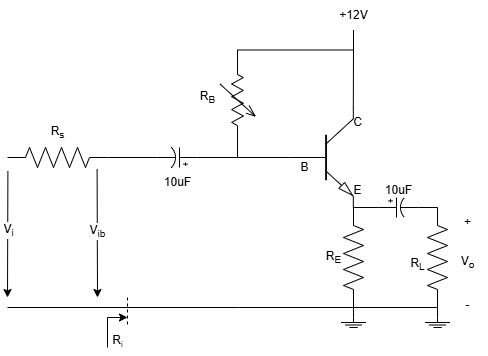
\includegraphics[width=0.7\linewidth]{Lab07/Lab7.drawio.png}
        \caption{A common-collector BJT amplifier/emitter follower.}
        \label{l7f}
    \end{figure}
    \FloatBarrier
In Fig.\ref{lab7f}, $V_{BEQ}$ = 0.6 V, $\beta$ = 160, $R_s$ = 10k$\Omega$, $R_B$ = 56k$\Omega$, $R_E$ = 1k$\Omega$.

\section{Detailed Procedures}
    \subsection{Analyzation}
    First, we analyze the circuit by drawing its AC-equivalent and DC-equivalent circuit.\par
    \begin{itemize}
        \item AC-equivalent Circuit:\par
            \begin{figure}[h]
                \centering
                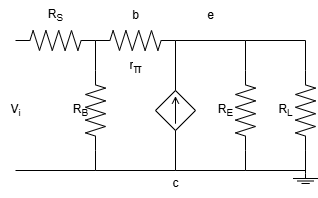
\includegraphics[width=0.65\linewidth]{Lab07/Lab7ac.drawio.png}
                \caption{AC-equivalent Circuit}
                \label{l7ac}
            \end{figure}
            \FloatBarrier
        \item DC-equivalent Circuit:\par
            \begin{figure}[h]
                \centering
                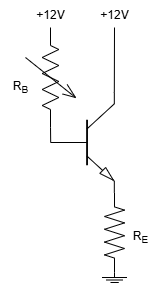
\includegraphics[width=0.3\linewidth]{Lab07/Lab7dc.drawio.png}
                \caption{DC-equivalent Circuit}
                \label{l7dc}
            \end{figure}
            \FloatBarrier
    \end{itemize}
    \FloatBarrier
    To analysis Fig.\ref{l7ac} and Fig.\ref{l7dc} with given data, we can obtain:\par
    In Fig.\ref{l6ac}\par
    \begin{equation}
        \begin{cases}
            R_{TH} = R_a//R_b\\
            V_{TH} = 12\cdot\frac{R_b}{R_a//R_b}\\
            12-i_cR_c-V_{CE}-i_ER_E=0\\
            V_{TH}-i_bR_{TH}-V_{BE}-i_eR_E=0\\
        \end{cases}
    \end{equation}
    
    In Fig.\ref{l6dc}\par
    \begin{equation}
        \begin{cases}
            A_v = \frac{V_i}{V_o} = \\
            R_i = R_B = 56k\\
            R_o = R_E//R_L = 1m\\
        \end{cases}
    \label{l6eq1}
    \end{equation}
    
    
    \subsection{Procedures}

    
\section{Discussion}


\section{Conclusion}
